\section{Methods of Classification}
	\subsection{Feature selection}
		\begin{frame}
			\frametitle{Scatterplots}
			We are looking for features with clustering
			\begin{columns}			
			\column[c]{.50\textwidth}
				\begin{figure}
					\centering
					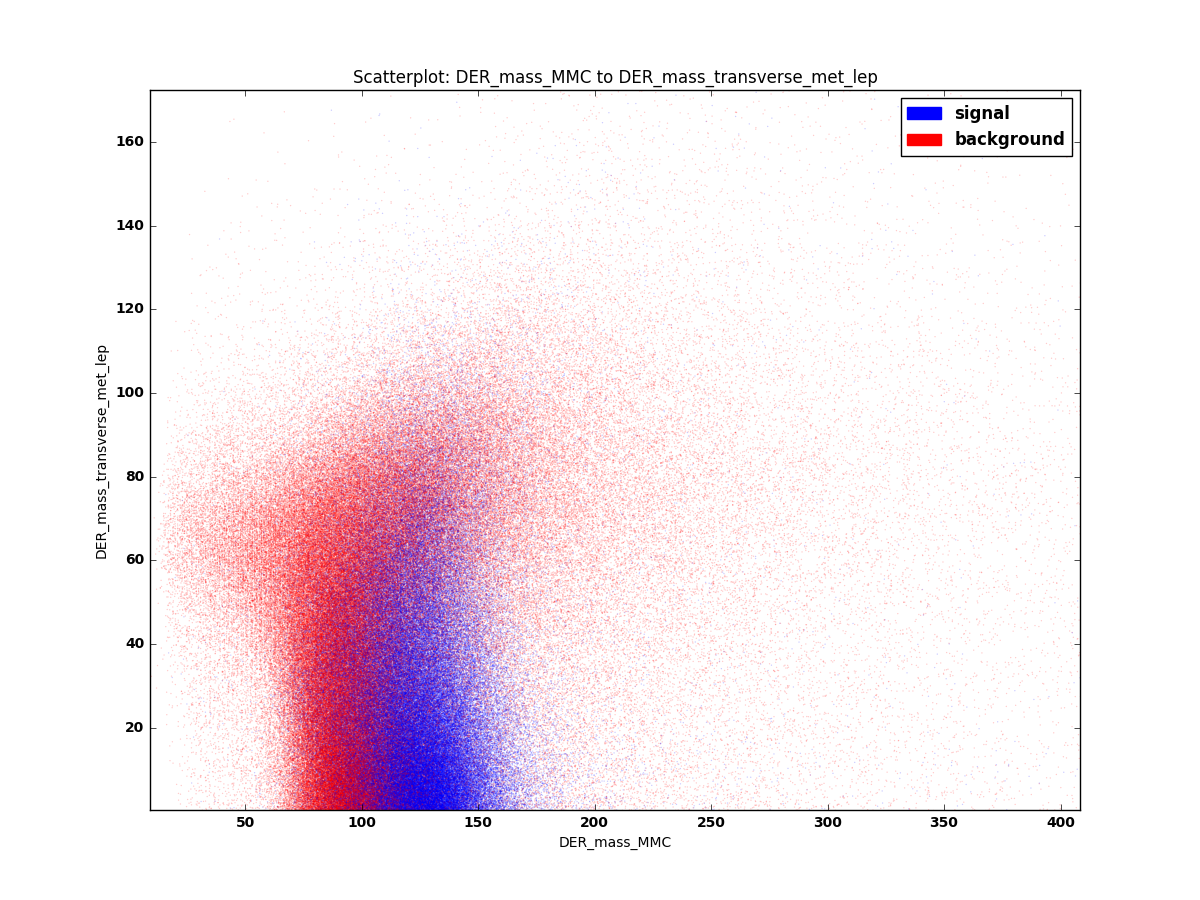
\includegraphics[width=130pt]{images/DER_mass_MMC}
					%\caption{Histogram of errors related to PRI\_jet\_num}
				\end{figure}
			\column[c]{.50\textwidth}
				\begin{figure}
					\centering
					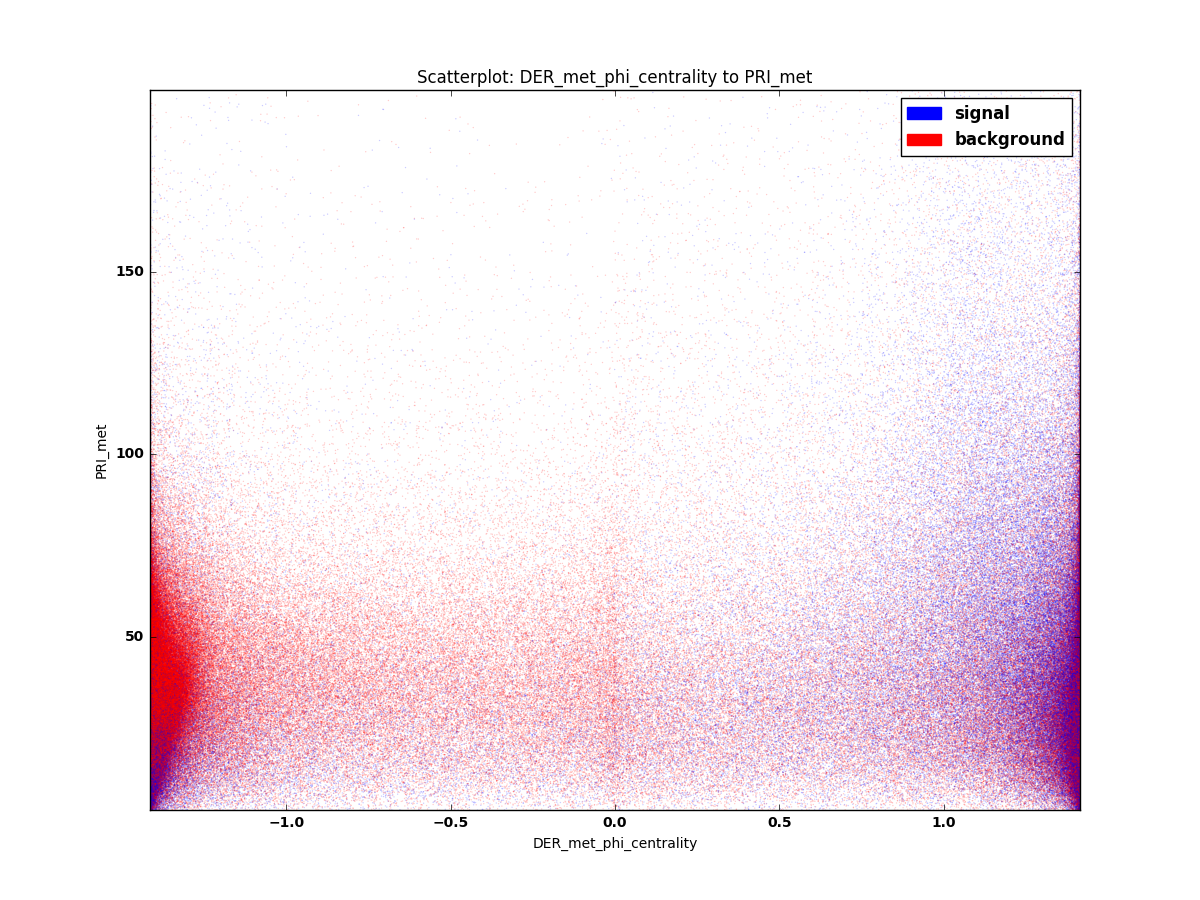
\includegraphics[width=130pt]{images/DER_met_phi_centrality}
					%\caption{Histogram of errors related to PRI\_jet\_num}
				\end{figure}
			\end{columns}	
		\end{frame}
		
		
		\begin{frame}
			\frametitle{Histograms}
			We are looking for good-separable signal-distribution
			\begin{columns}			
			\column[c]{.50\textwidth}
				\begin{figure}
					\centering
					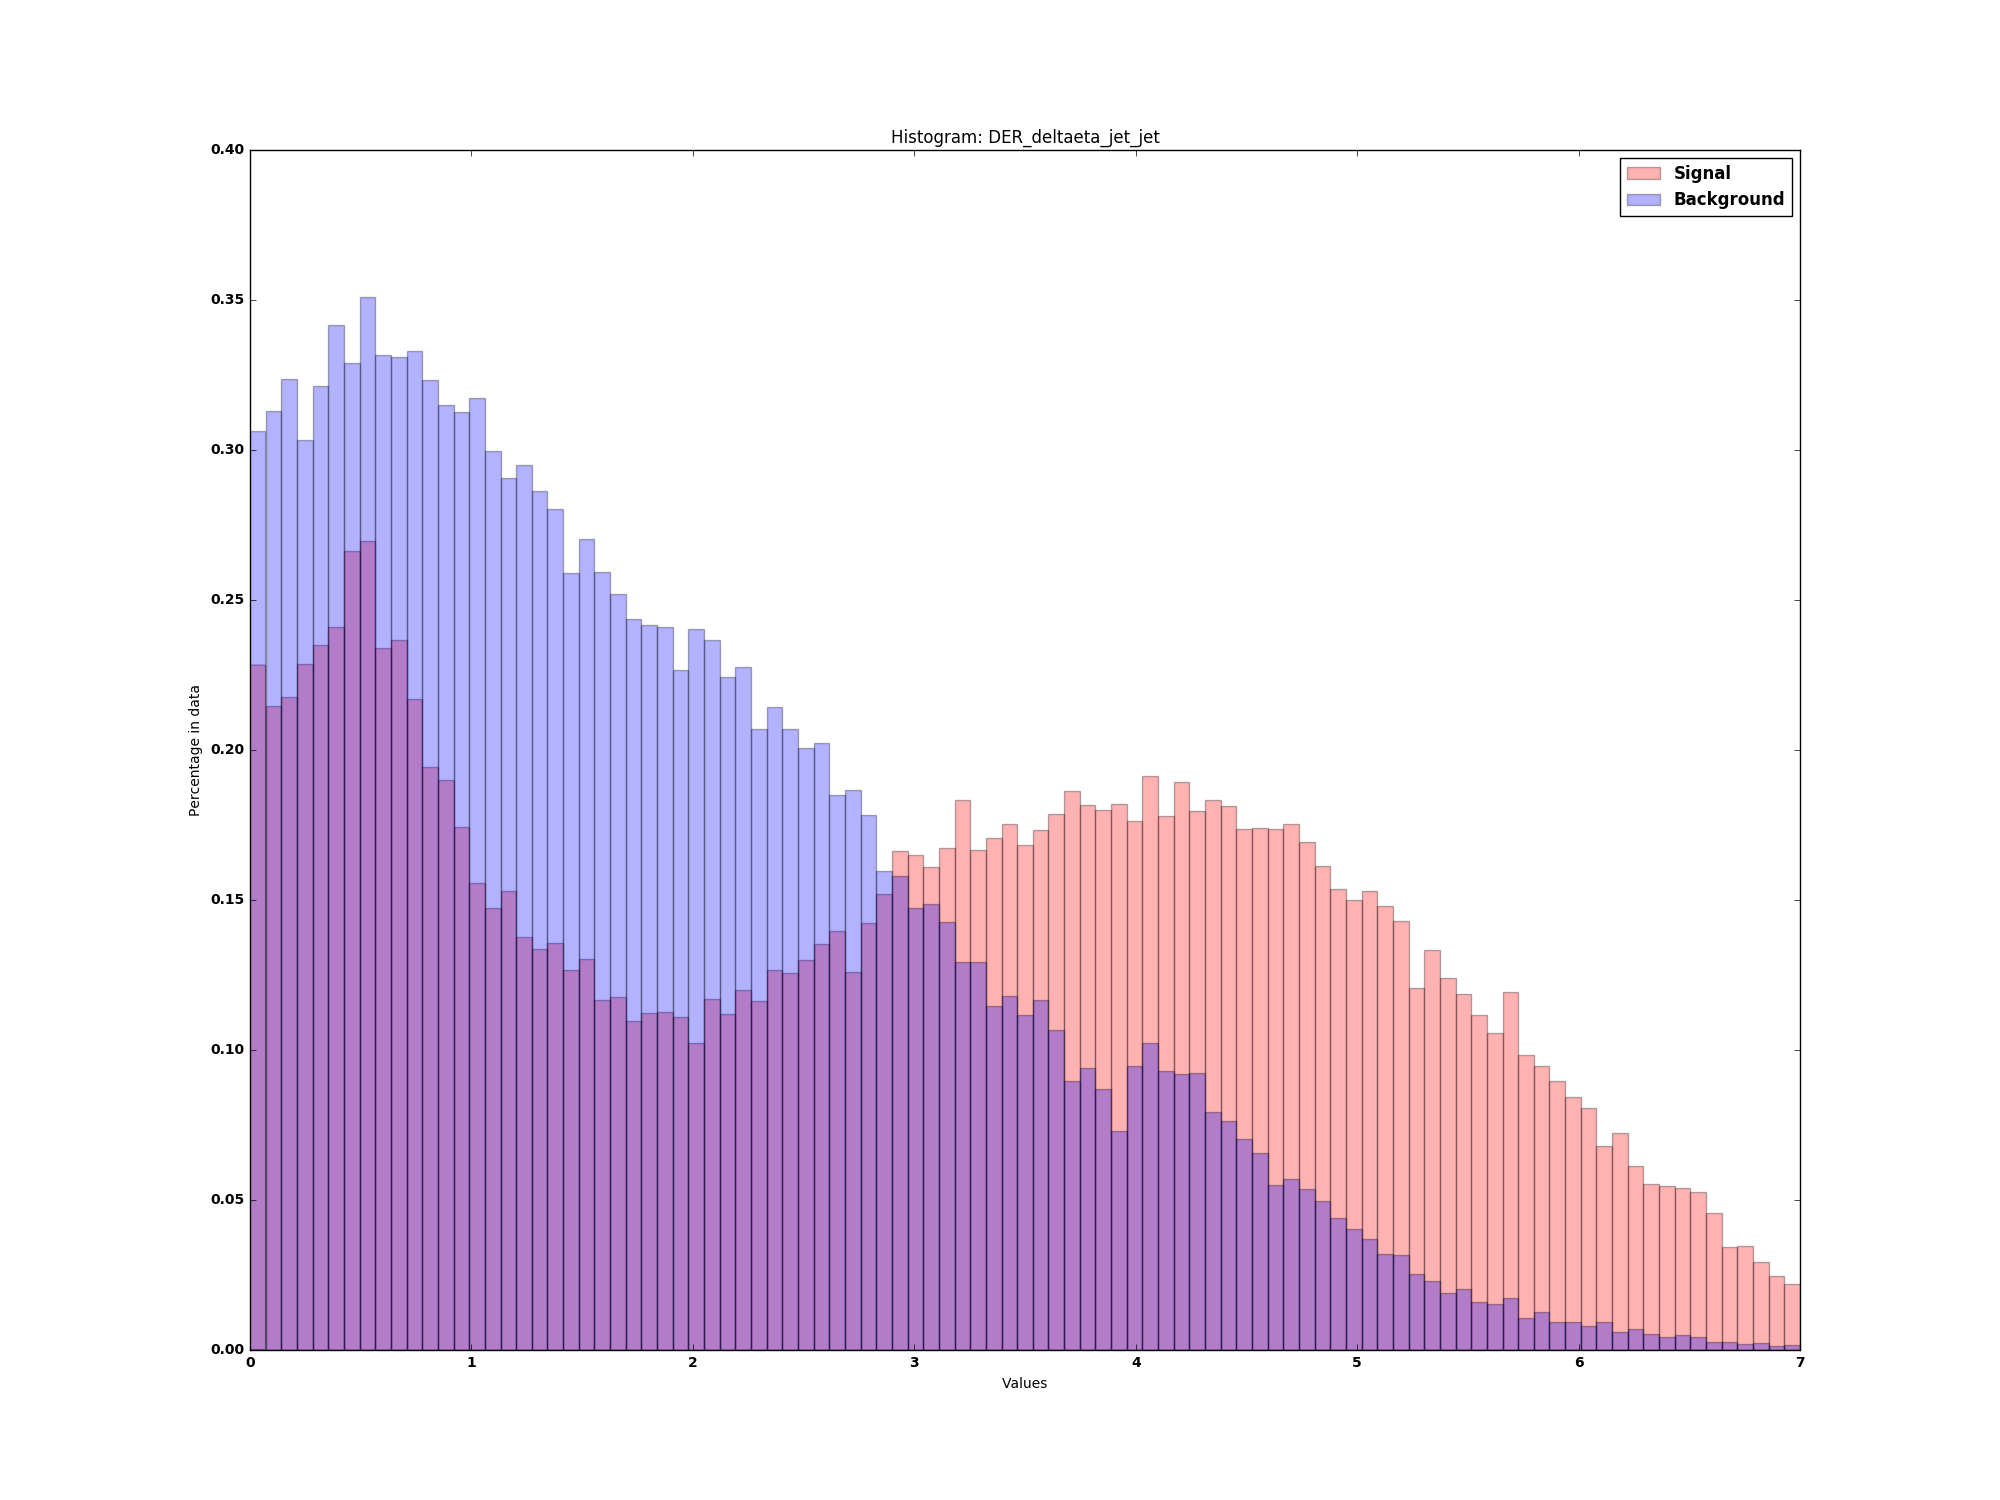
\includegraphics[width=130pt]{images/DER_deltaeta_jet_jet}
					%\caption{Histogram of errors related to PRI\_jet\_num}
				\end{figure}
			\column[c]{.50\textwidth}
				\begin{figure}
					\centering
					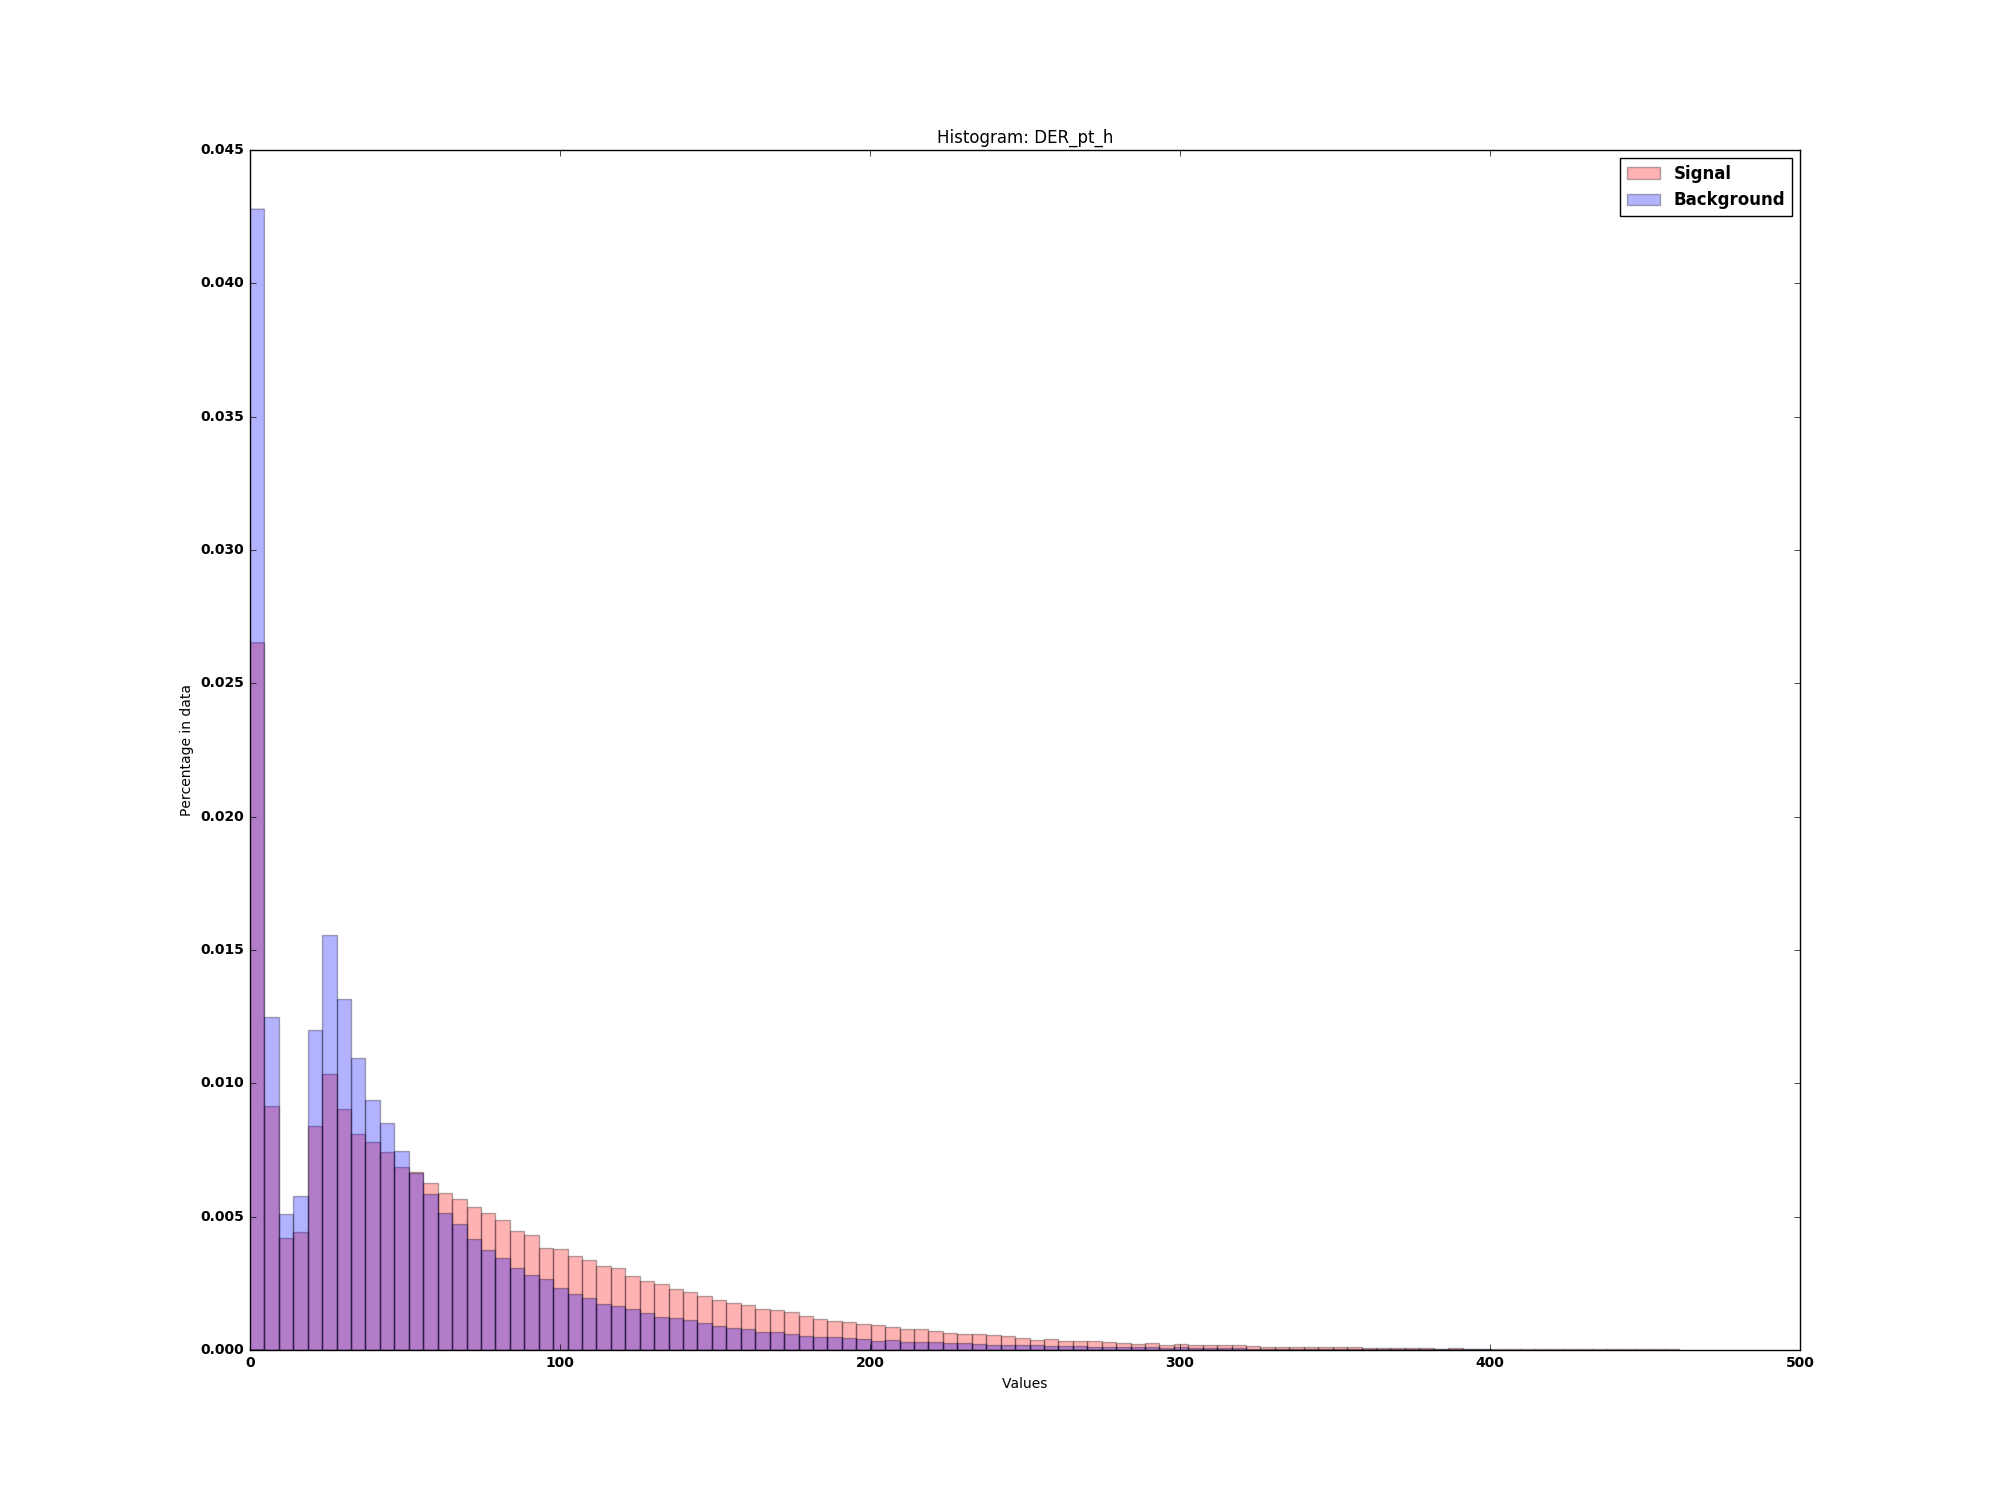
\includegraphics[width=130pt]{images/hist_DER_pt_h}
					%\caption{Histogram of errors related to PRI\_jet\_num}
				\end{figure}
			\end{columns}
		\end{frame}
		
		\begin{frame}
			\frametitle{PRI\_jet\_num and error-values}
			\begin{columns}			
			\column[c]{.50\textwidth}
			\only<1>{
				\begin{itemize}
					\item 62\% of events contain features with value $-999.0$
					\item No flaw of simulation, but values are 
						  \textit{structurally absent}
				\end{itemize}
			}
			
			\only<2>{
				\begin{quote}
					"For instance, in events where there is no jet 
					[...], there is no such a thing as a “leading 
					jet”, thus the associated quantities [...] are
					structurally undefined, and the features derived from these 
					as well." \cite{germainForum}
				\end{quote}
			}
			
			\only<3>{
				\begin{quote}
					"In fact, all missing features are related to 
					PRI\_jet\_num, except DER\_mass\_MMC." \cite{germainForum}
				\end{quote}
				
				We conclude, that seven features contain no information for
				~25\% of events. It will help us to optimize our classifiers.
			}

				
				
			\column[c]{.50\textwidth}
				\begin{figure}
					\centering
					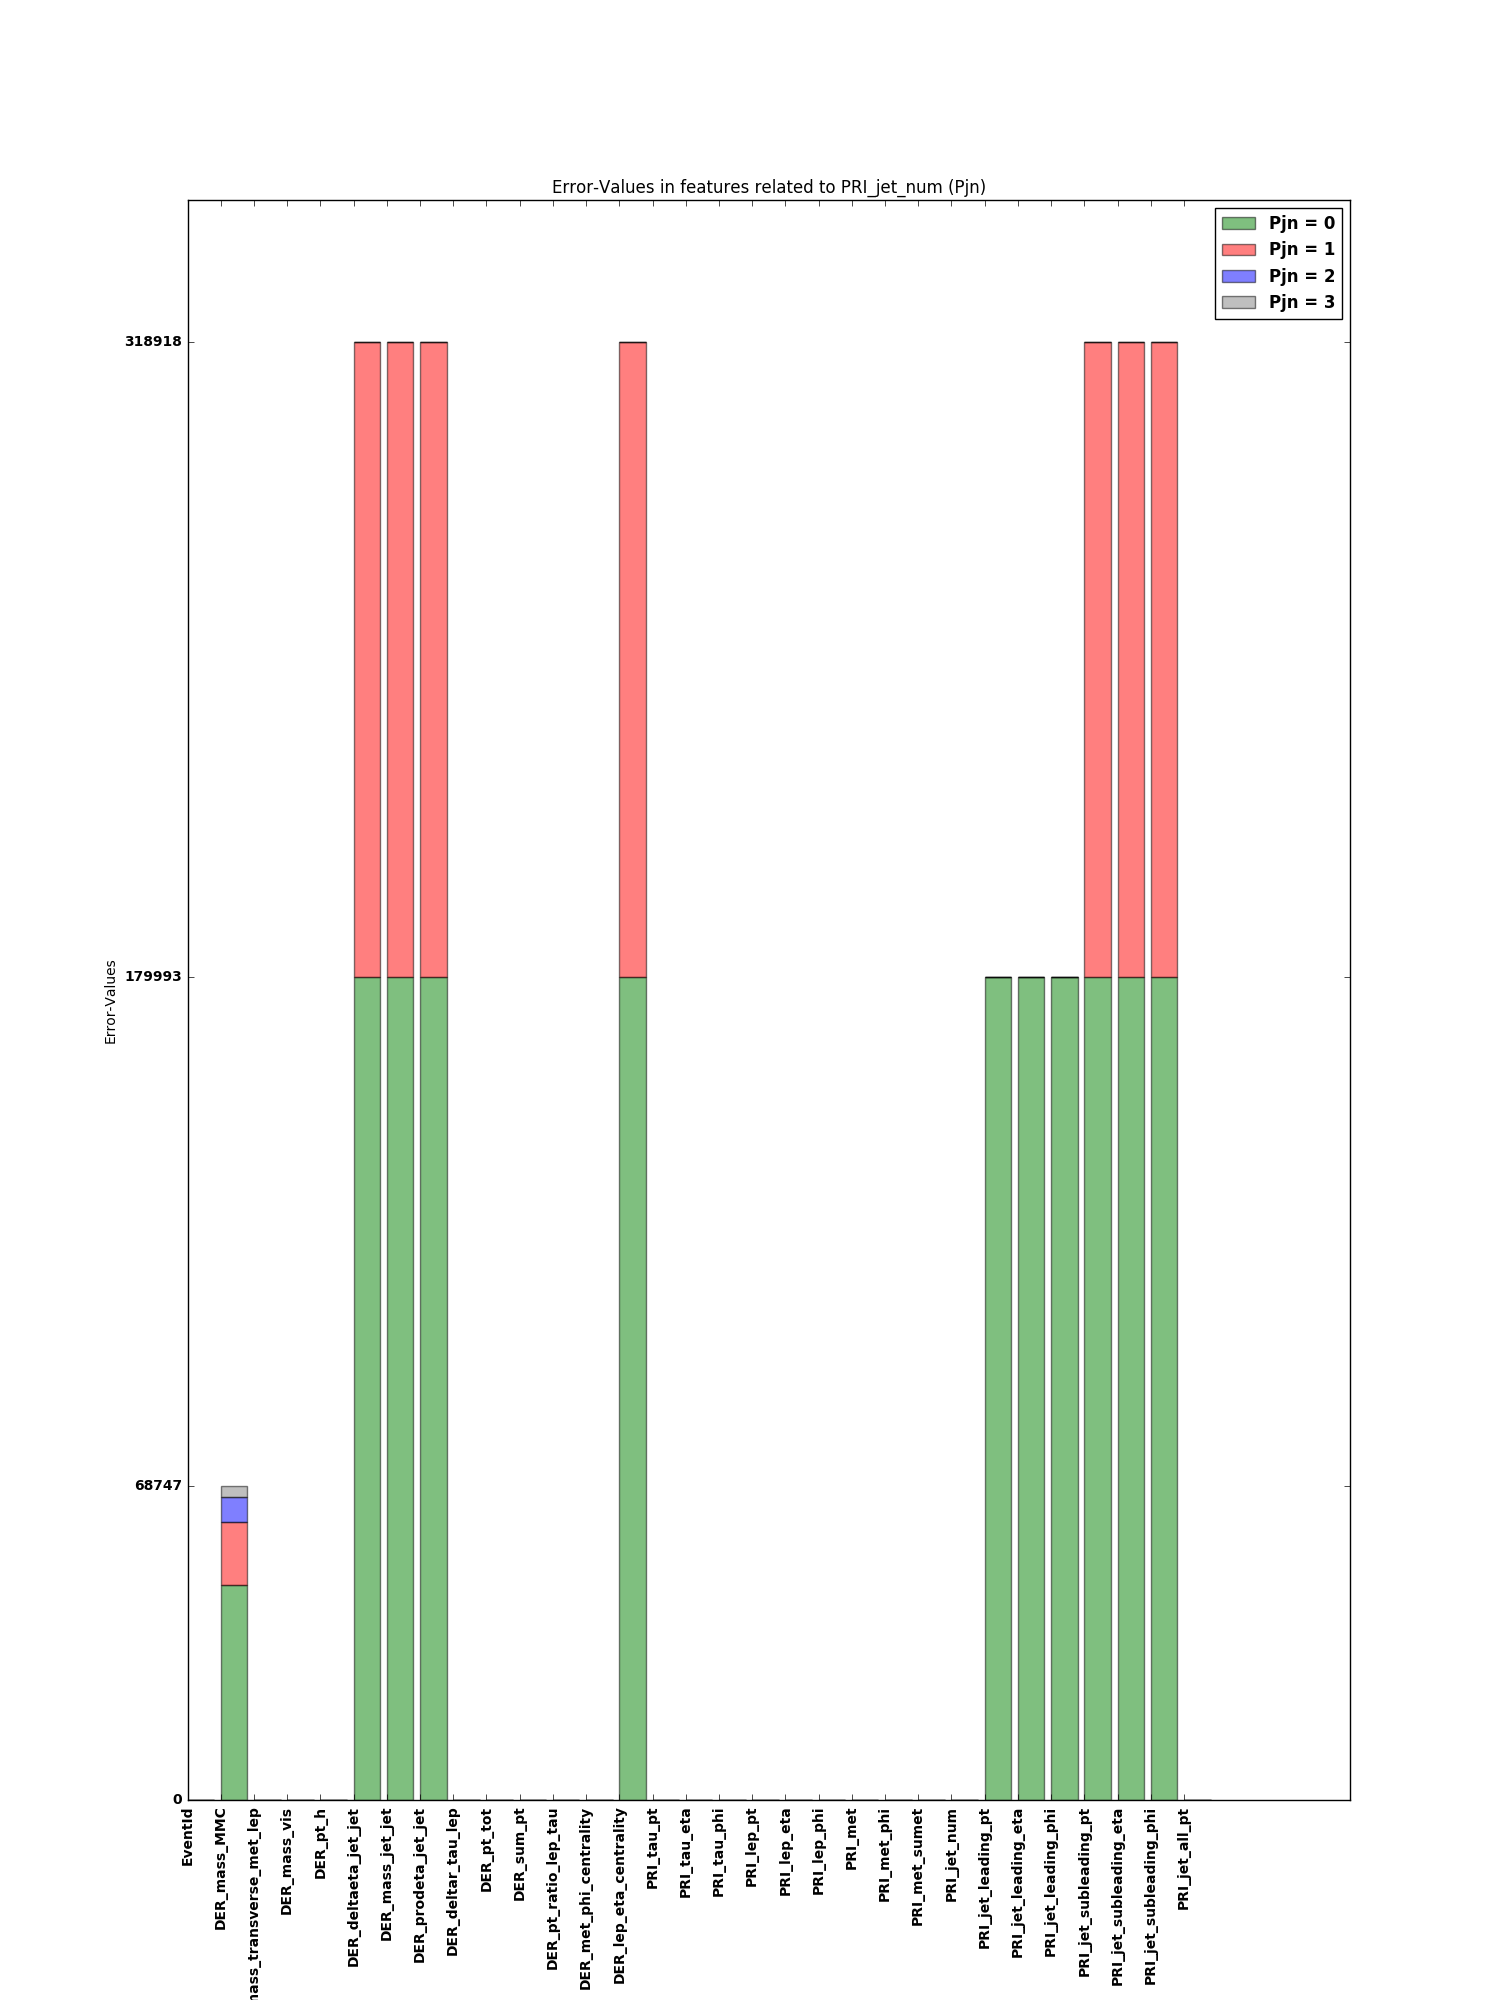
\includegraphics[width=130pt]{images/PJN_Errors}
					\caption{Histogram of errors related to PRI\_jet\_num}
				\end{figure}
			\end{columns}			
		\end{frame}
		
		
		
	\subsection{Logistic regression}
		\begin{frame}
			%\frametitle{Logistic regression}
			\centering
			Logistic Regression
		\end{frame}	
	
	
		\begin{frame}
			\frametitle{Logistic regression - Score}
			\centering
			First, we try only few features.
			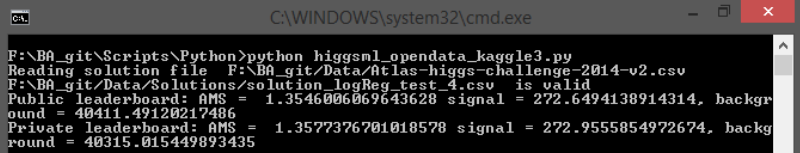
\includegraphics[scale=0.5]{images/logReg_ams_4}
			Really low AMS, we would make rank 1625
		\end{frame}
		
		\begin{frame}
			\frametitle{Logistic regression - Score}
			\centering
			We simply use all our data and normalize it
			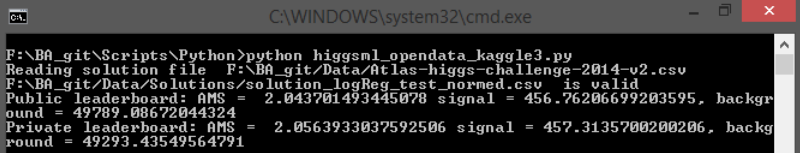
\includegraphics[scale=0.5]{images/logReg_ams}
			\\(matches with rank 1473)
		\end{frame}

	\subsection{k-Nearest-Neighbours}
		\begin{frame}
			%\frametitle{k-Nearest-Neighbours}
			\centering
			k-Nearest-Neighbours
		\end{frame}
		
		\begin{frame}
			\frametitle{k-Nearest-Neighbours - Score}
			\centering
			Again, we simply use all our data\\
			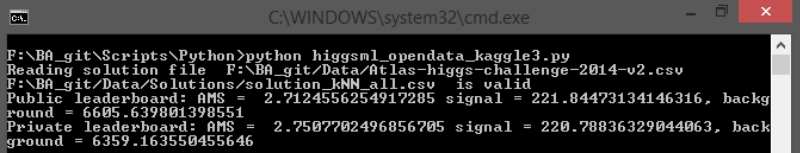
\includegraphics[scale=0.5]{images/kNN_ams_all}
			\\Not very exciting \ldots
			Also kNN rapidly slows down with increasing feature number, we should 
			remove "bad" features.
		\end{frame}
		
		\begin{frame}
			\frametitle{k-Nearest-Neighbours - Score}
			\centering
			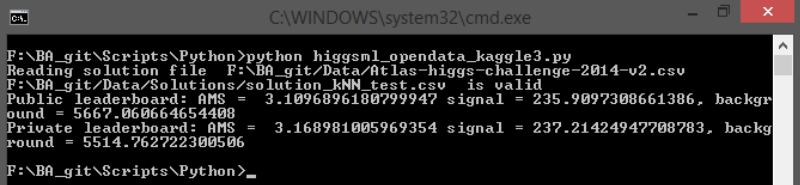
\includegraphics[scale=0.5]{images/kNN_ams}
			\\HOLY AMS, BATMAN!
			\only<2>{\\(regarding the challenge, this would place us on rank 998)
			}
		\end{frame}